\section{Anhang Schema}\label{sec:appendix_schema}

%%%%%%%%%%%%%%%%%%%%%%%%%%%%%%%%%%%%%%%%%%%%%%%%%%%%%%%%%%%%%%%%%%%%%%%%%%%%%%%%
% pictures
\begin{figure}[htb]
\begin{center}
\includegraphics[width=\textwidth]{graphics/image_appendix_schematic.png}
\end{center}
\caption{Schema} % picture caption
\label{fig:image_print_output_schematic_overview}
\end{figure}
%
%(Abb. \ref{fig:image1})
%%%%%%%%%%%%%%%%%%%%%%%%%%%%%%%%%%%%%%%%%%%%%%%%%%%%%%%%%%%%%%%%%%%%%%%%%%%%%%%%
\clearpage

%%%%%%%%%%%%%%%%%%%%%%%%%%%%%%%%%%%%%%%%%%%%%%%%%%%%%%%%%%%%%%%%%%%%%%%%%%%%%%%%
% pictures
\begin{figure}[htb]
\begin{center}
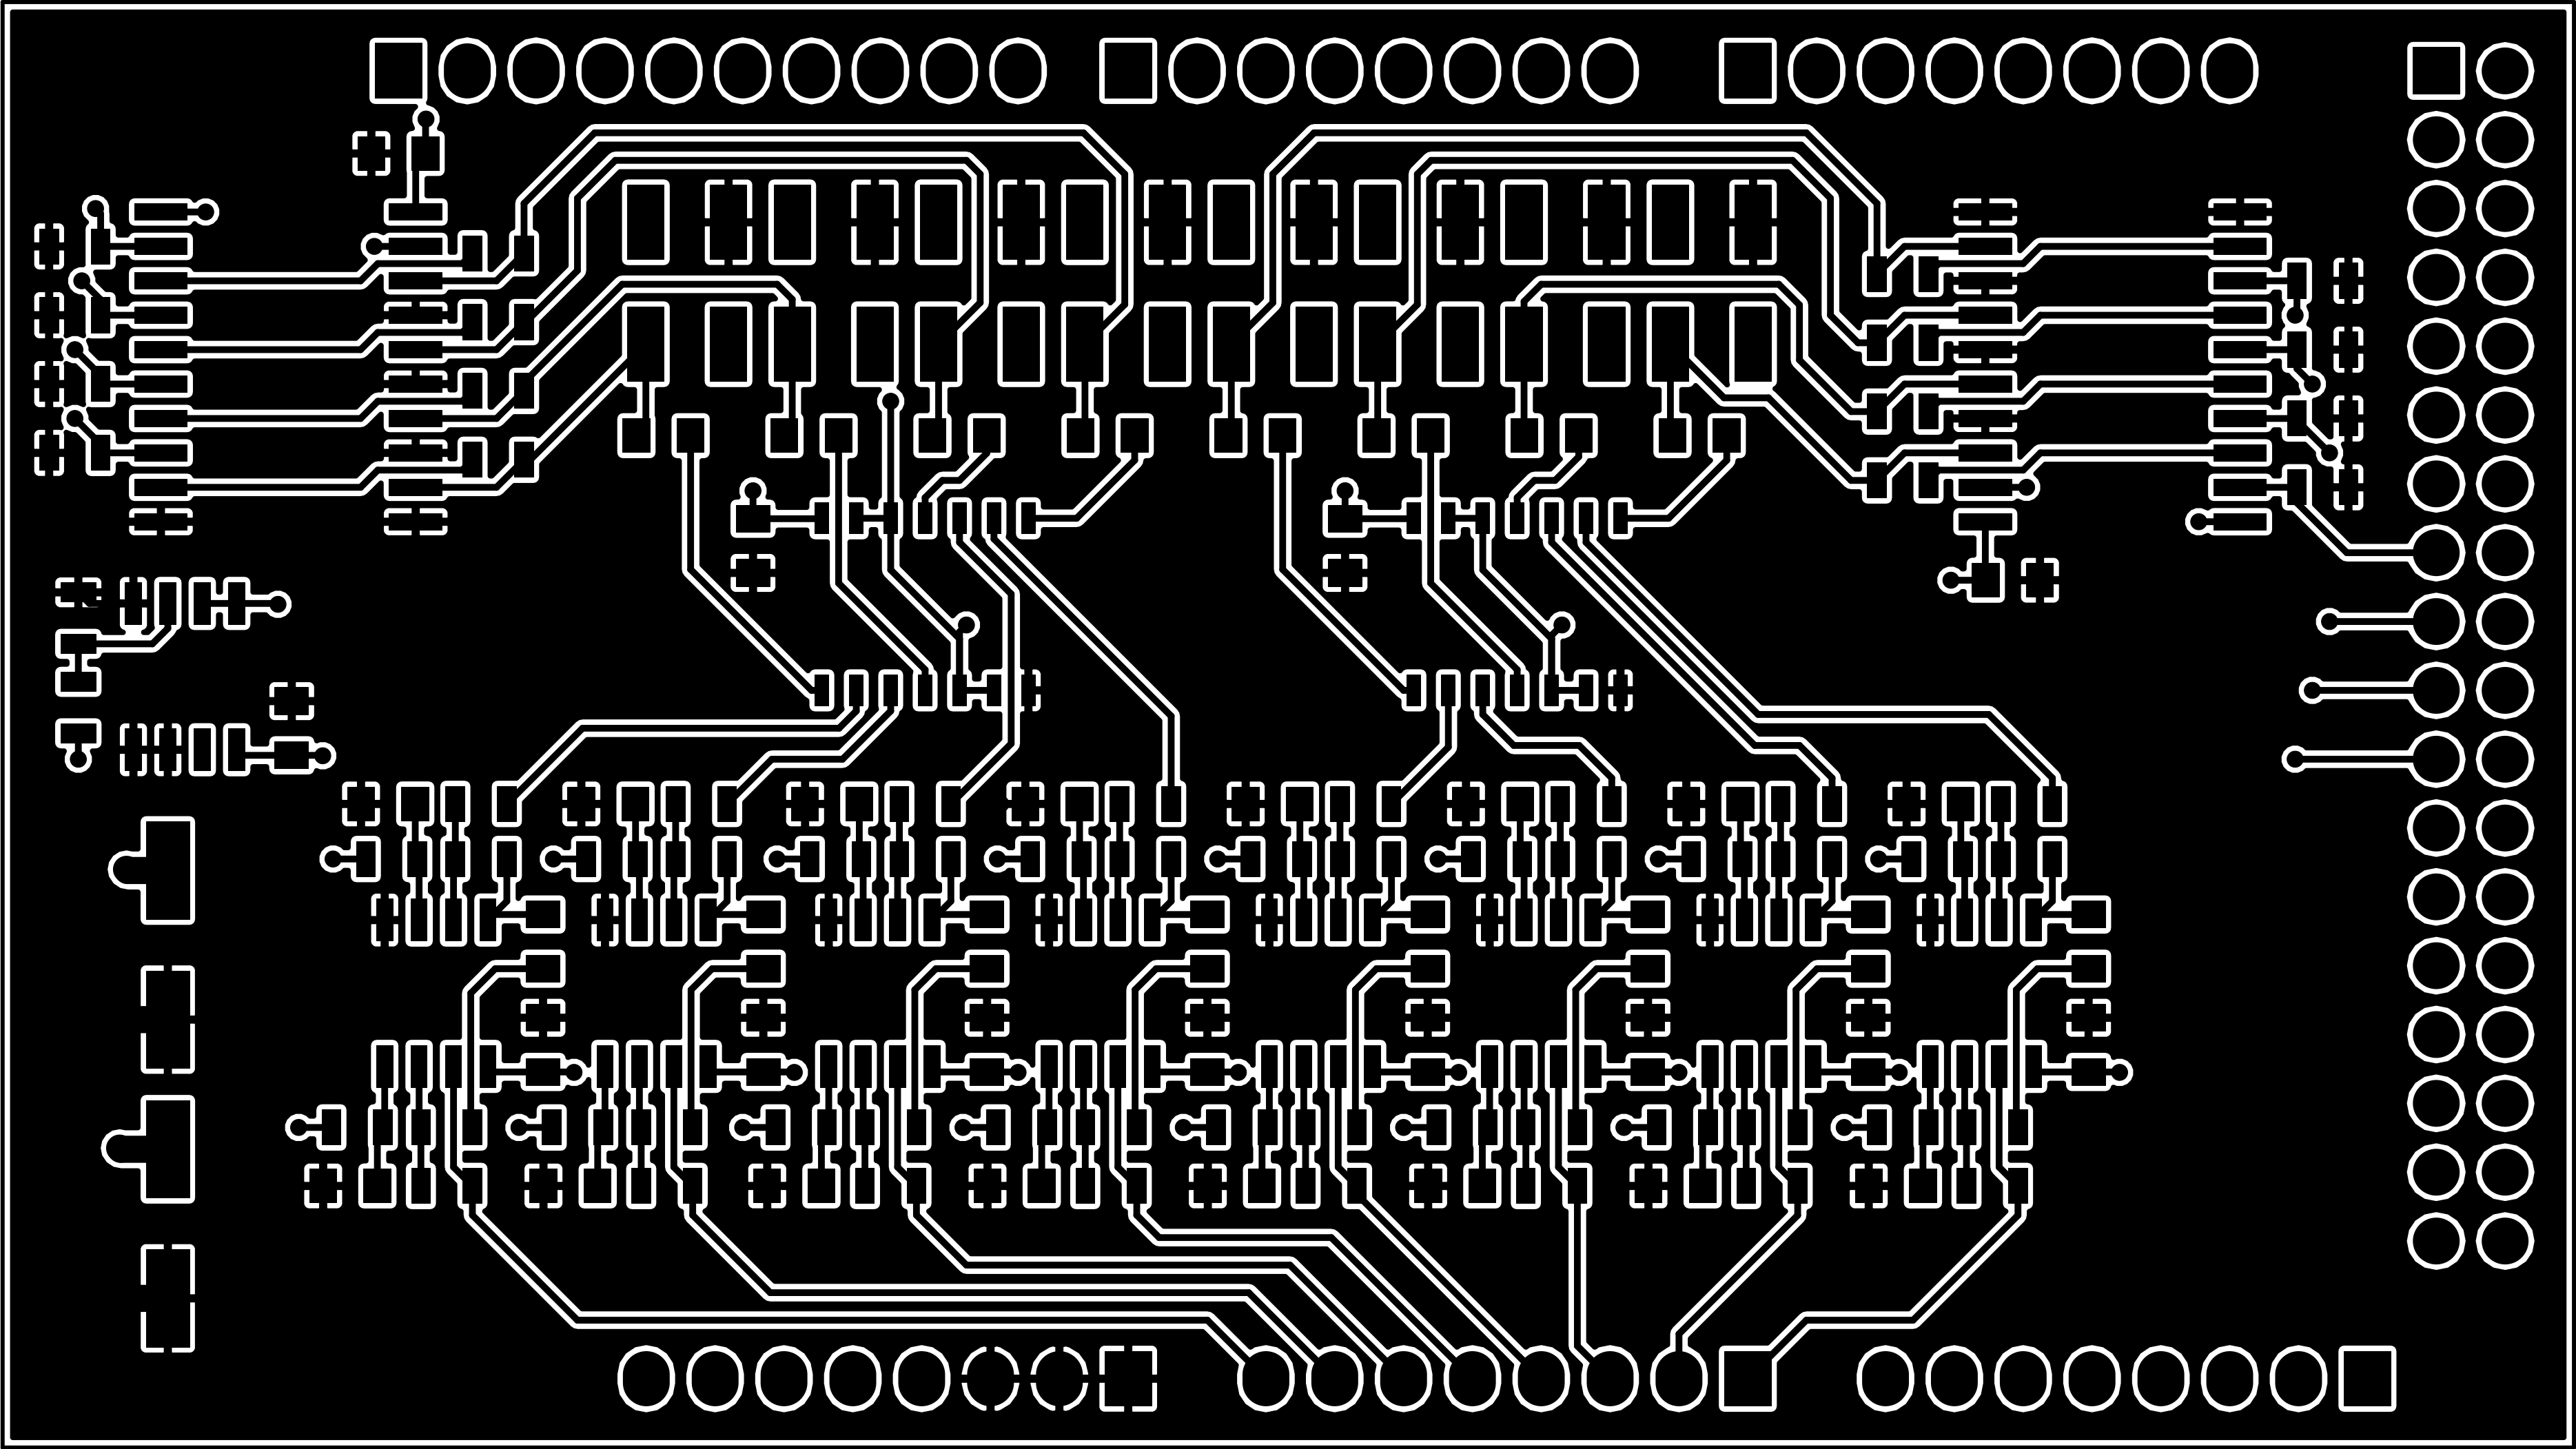
\includegraphics[width=0.9\textwidth]{graphics/image_appendix_copper_top.png}
\end{center}
\caption{Top Copper (signal)} % picture caption
\label{fig:image_appendix_copper_top}
\end{figure}
%
%(Abb. \ref{fig:image1})
%%%%%%%%%%%%%%%%%%%%%%%%%%%%%%%%%%%%%%%%%%%%%%%%%%%%%%%%%%%%%%%%%%%%%%%%%%%%%%%%

%%%%%%%%%%%%%%%%%%%%%%%%%%%%%%%%%%%%%%%%%%%%%%%%%%%%%%%%%%%%%%%%%%%%%%%%%%%%%%%%
% pictures
\begin{figure}[htb]
\begin{center}
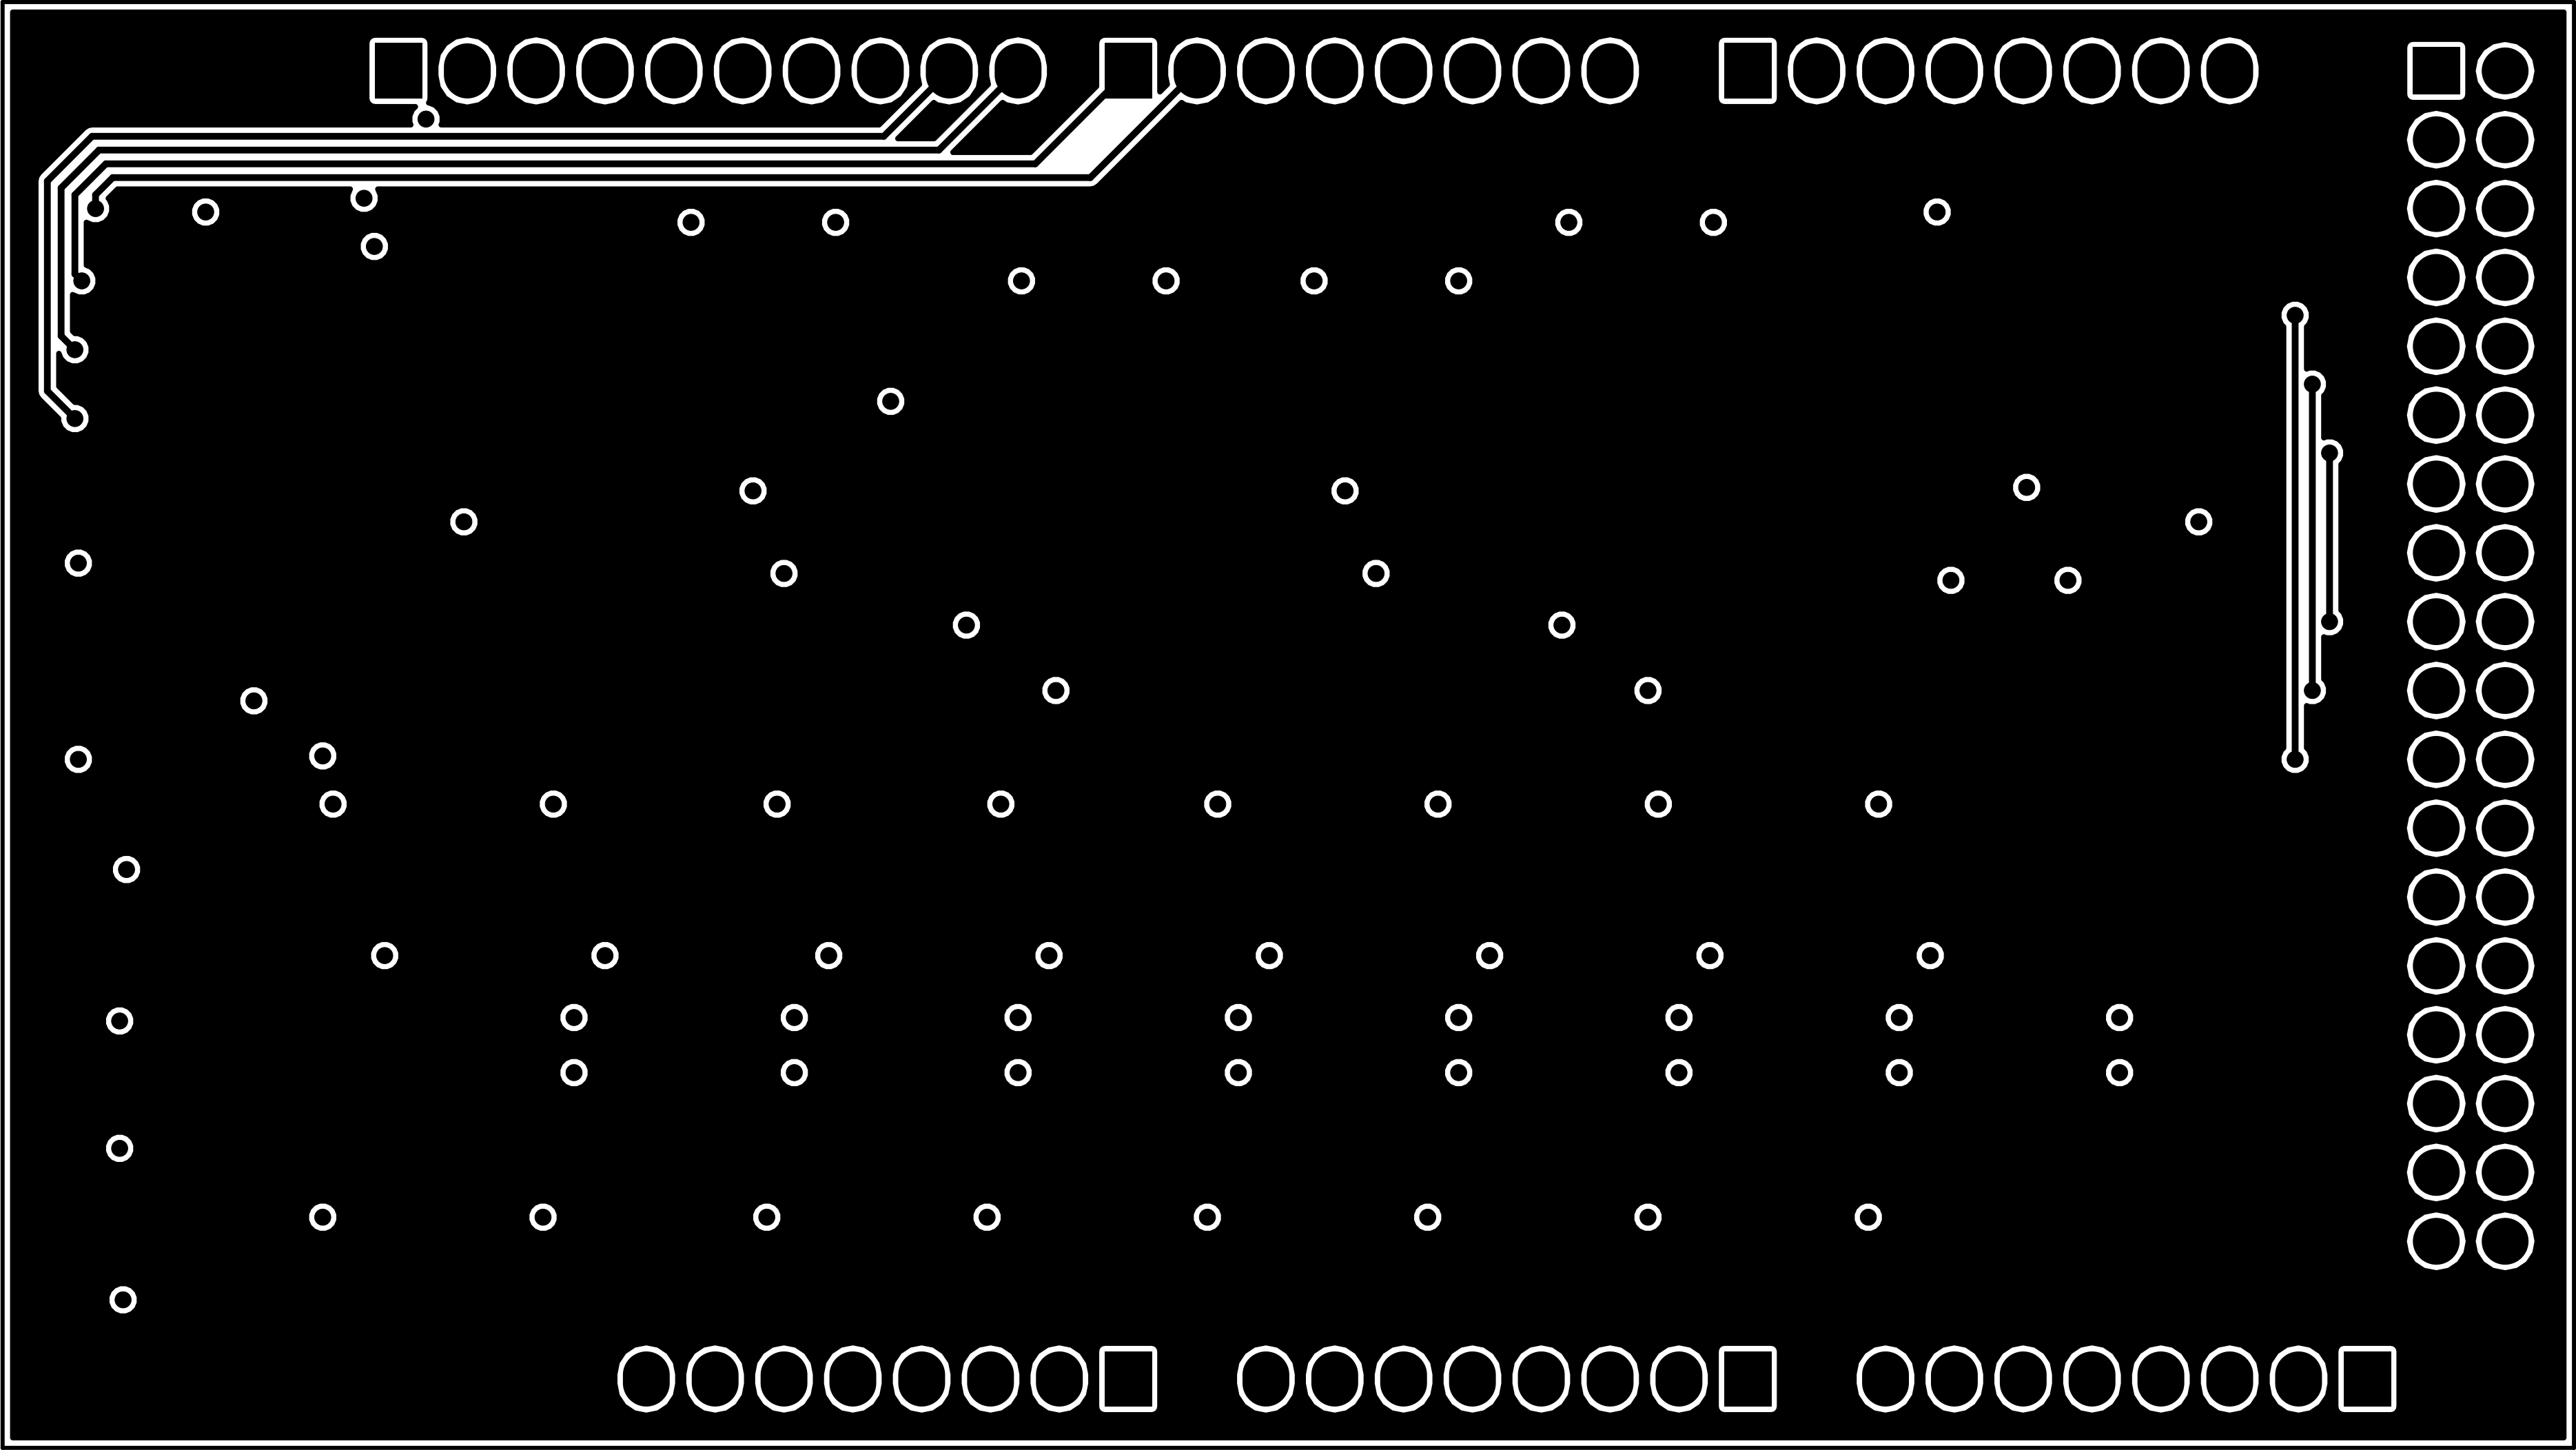
\includegraphics[width=0.9\textwidth]{graphics/image_appendix_copper_1.png}
\end{center}
\caption{Inner Layer 1 (virtual ground 1.65V)} % picture caption
\label{fig:image_appendix_copper_1}
\end{figure}
%
%(Abb. \ref{fig:image1})
%%%%%%%%%%%%%%%%%%%%%%%%%%%%%%%%%%%%%%%%%%%%%%%%%%%%%%%%%%%%%%%%%%%%%%%%%%%%%%%%

\clearpage
%%%%%%%%%%%%%%%%%%%%%%%%%%%%%%%%%%%%%%%%%%%%%%%%%%%%%%%%%%%%%%%%%%%%%%%%%%%%%%%%
% pictures
\begin{figure}[htb]
\begin{center}
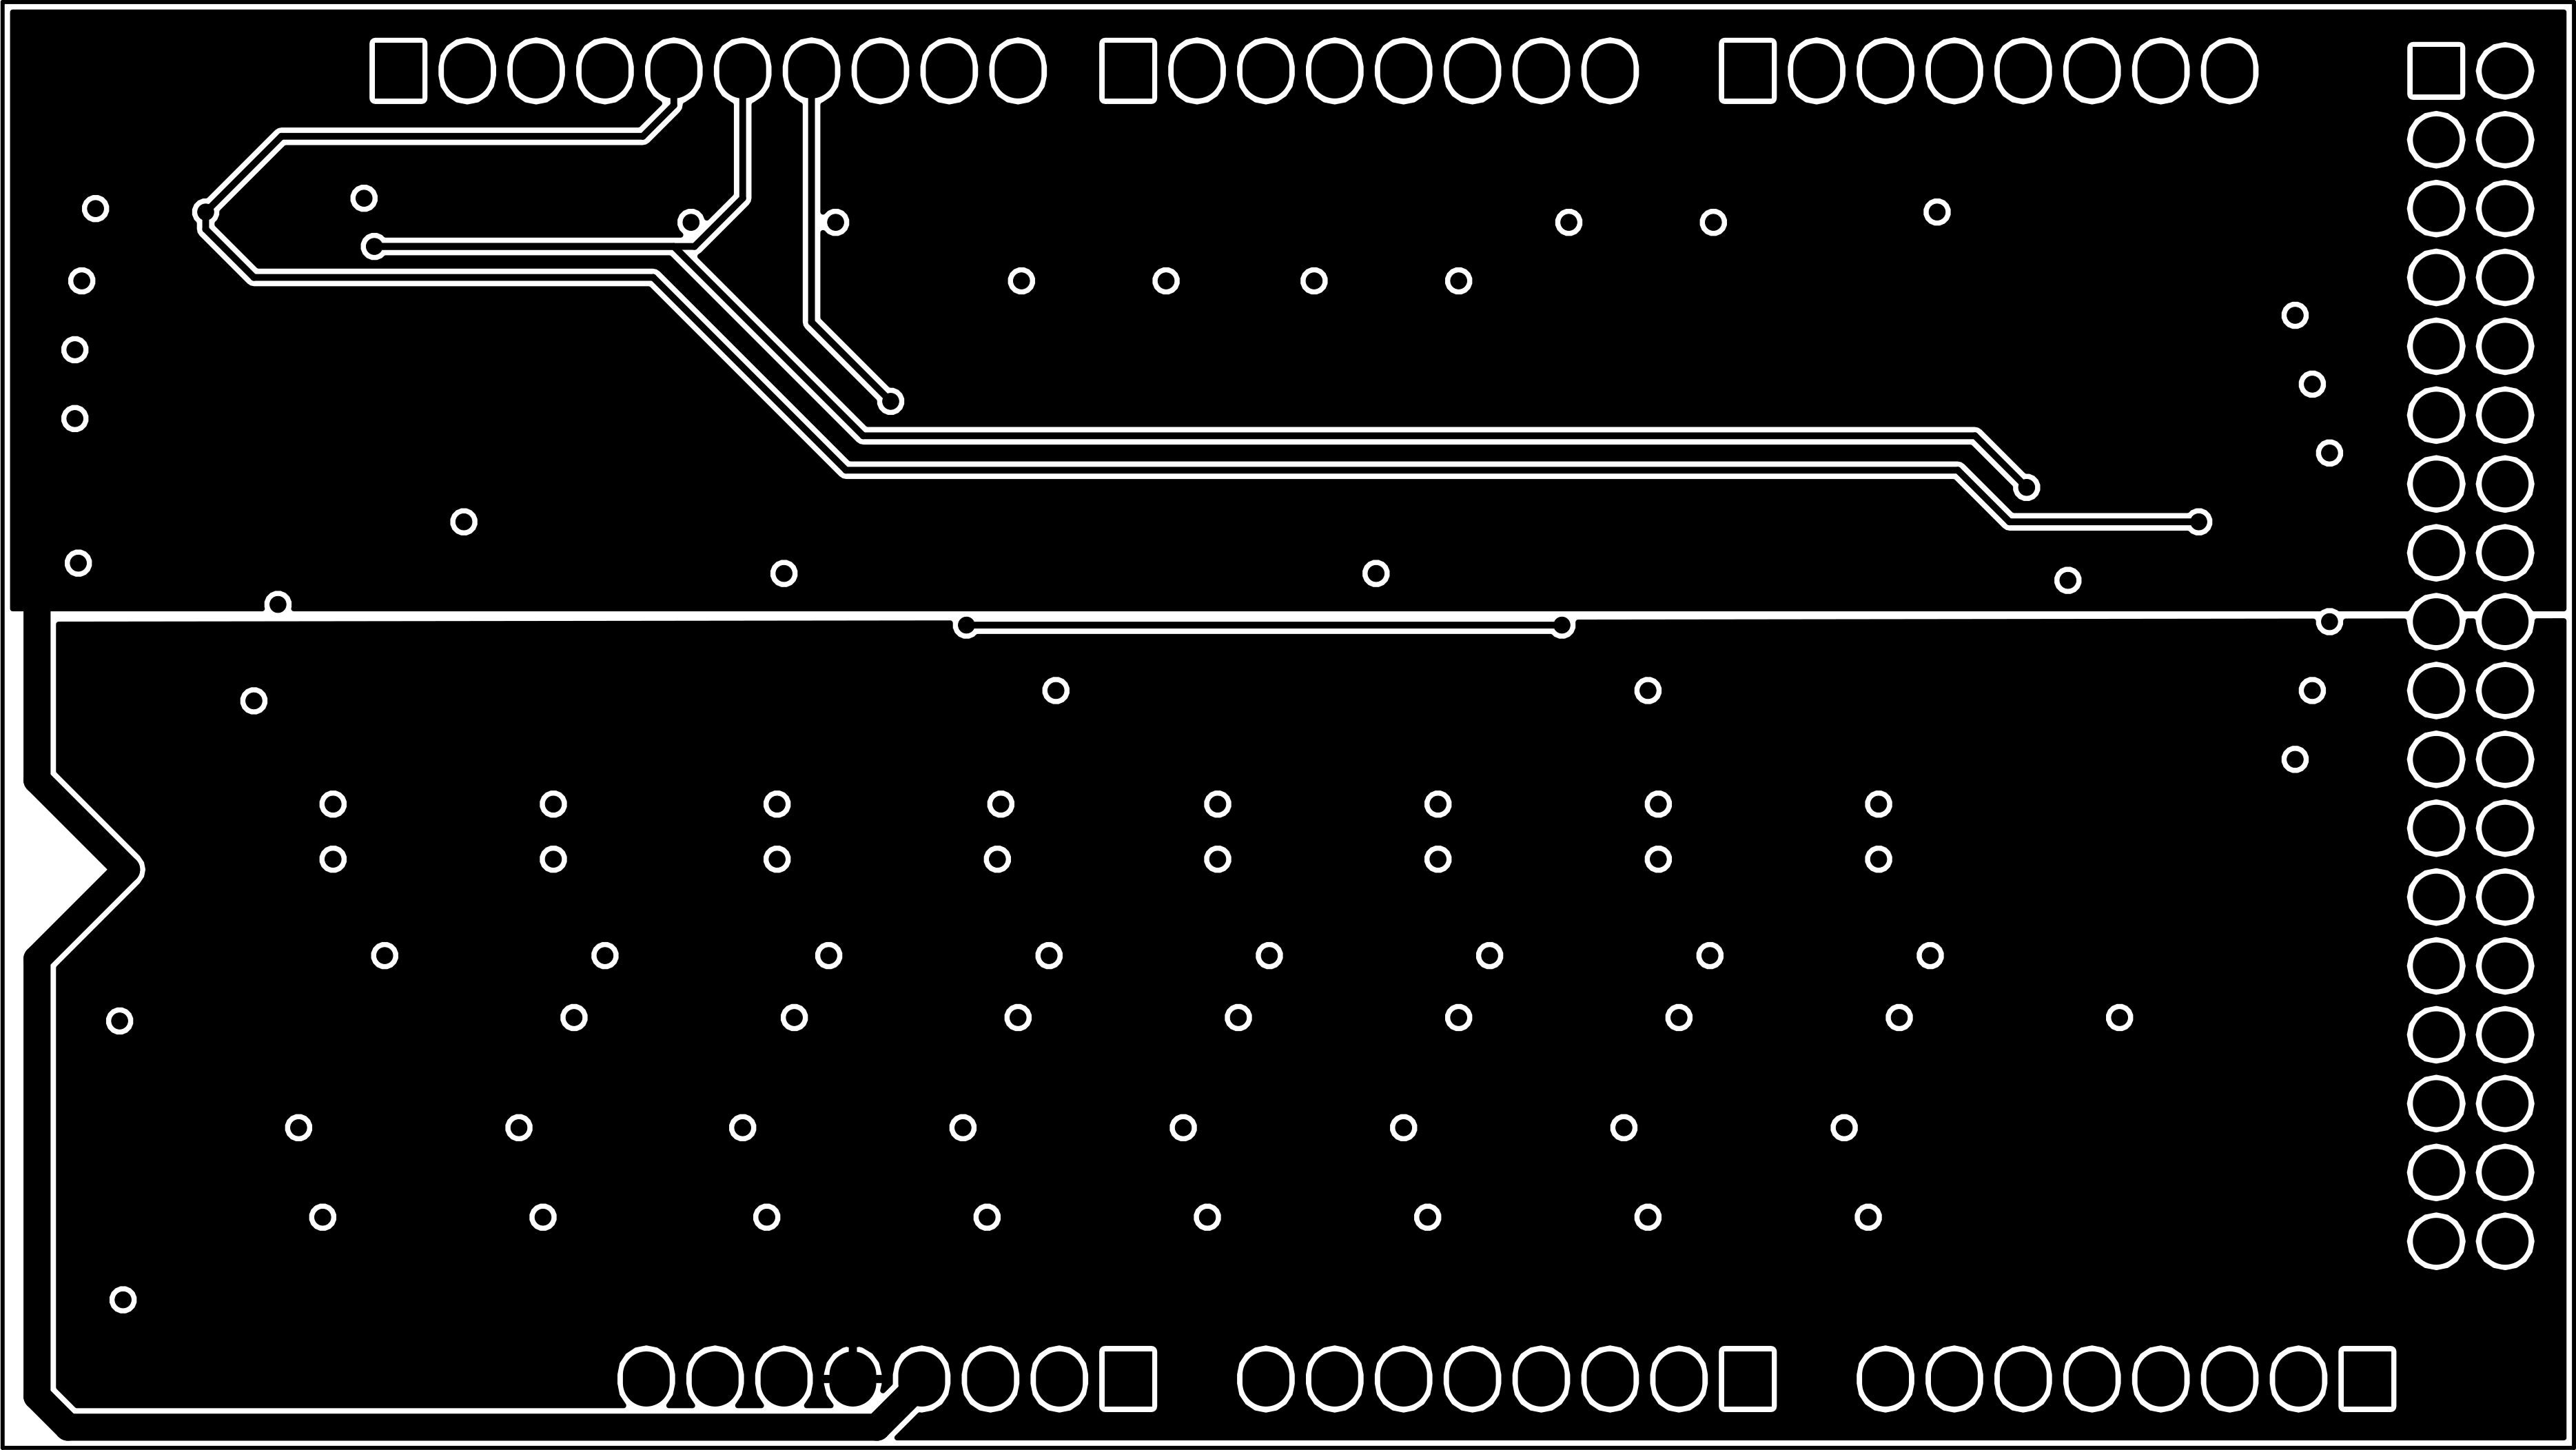
\includegraphics[width=0.9\textwidth]{graphics/image_appendix_copper_2.png}
\end{center}
\caption{Inner Layer 2 (VCC 5.0V, VCC 3.3V)} % picture caption
\label{fig:image_appendix_copper_2}
\end{figure}
%
%(Abb. \ref{fig:image1})
%%%%%%%%%%%%%%%%%%%%%%%%%%%%%%%%%%%%%%%%%%%%%%%%%%%%%%%%%%%%%%%%%%%%%%%%%%%%%%%%

%%%%%%%%%%%%%%%%%%%%%%%%%%%%%%%%%%%%%%%%%%%%%%%%%%%%%%%%%%%%%%%%%%%%%%%%%%%%%%%%
% pictures
\begin{figure}[htb]
\begin{center}
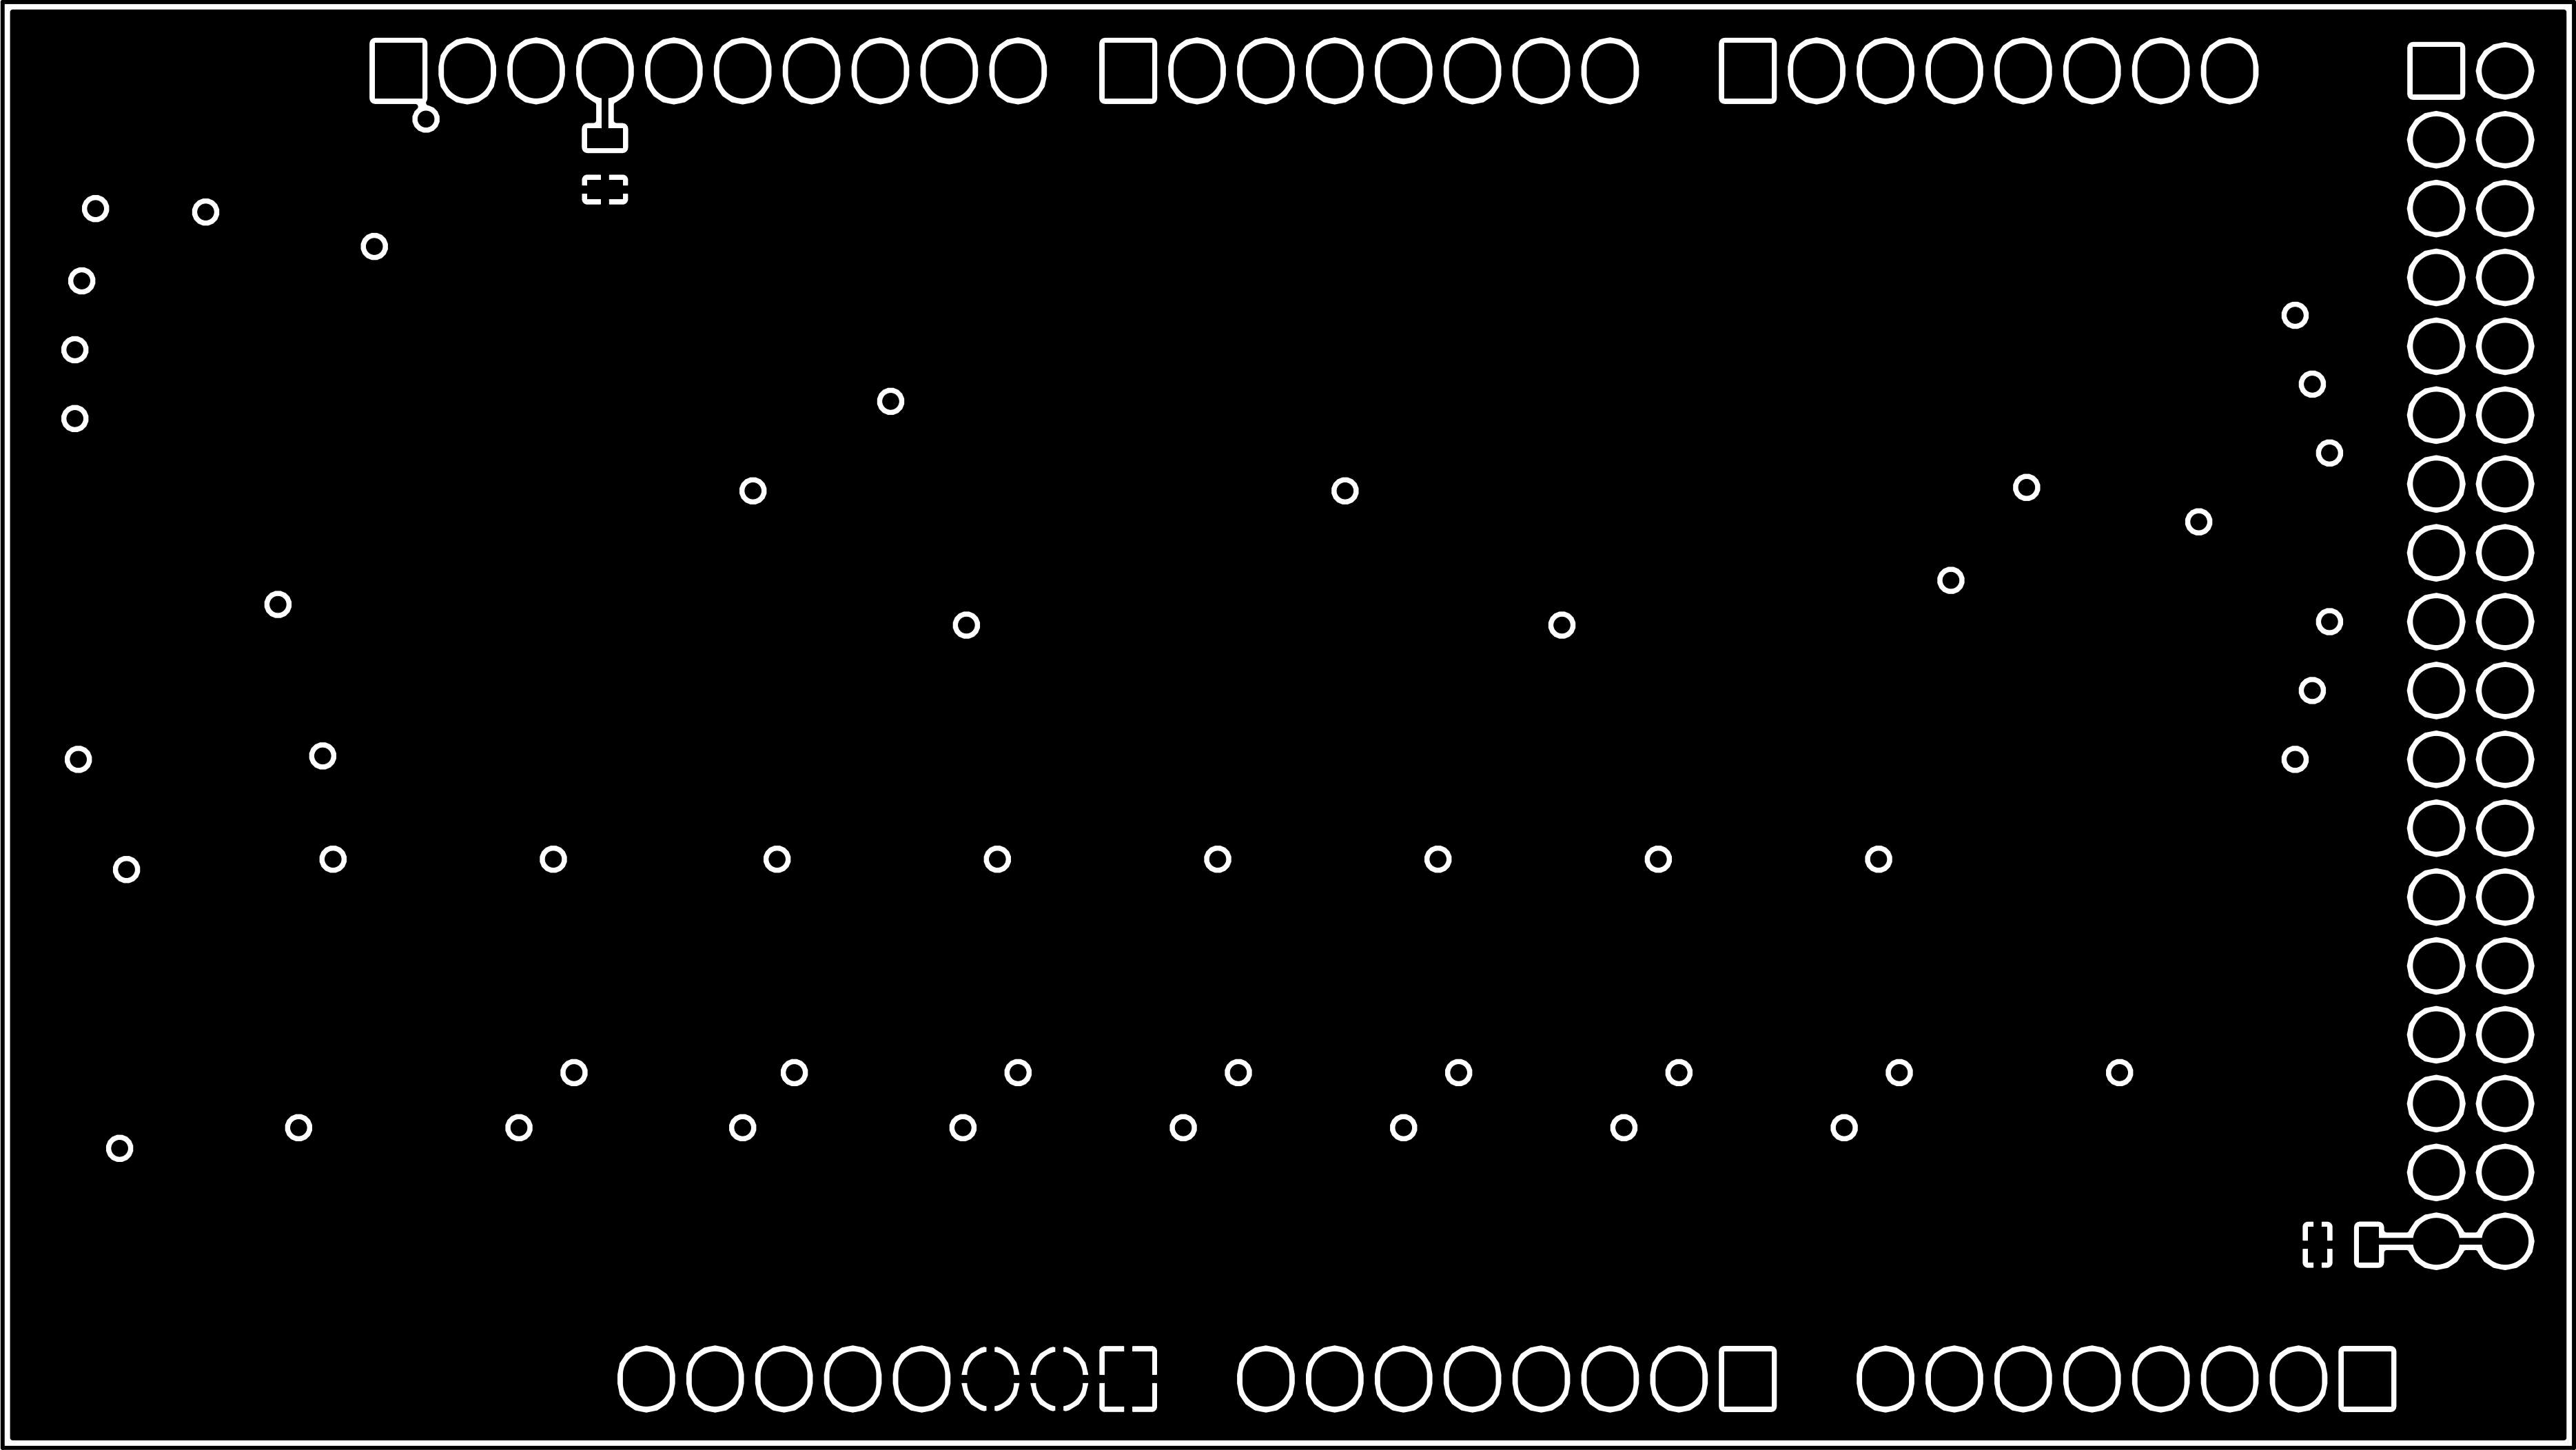
\includegraphics[width=0.9\textwidth]{graphics/image_appendix_copper_bottom.png}
\end{center}
\caption{Bottom Copper (ground)} % picture caption
\label{fig:image_appendix_copper_bottom}
\end{figure}
%
%(Abb. \ref{fig:image1})
%%%%%%%%%%%%%%%%%%%%%%%%%%%%%%%%%%%%%%%%%%%%%%%%%%%%%%%%%%%%%%%%%%%%%%%%%%%%%%%%



\clearpage
%%%%%%%%%%%%%%%%%%%%%%%%%%%%%%%%%%%%%%%%%%%%%%%%%%%%%%%%%%%%%%%%%%%%%%%%%%%%%%%%
%%%%%%%%%%%%%%%%%%%%%%%%%%%%%%%%%%%%%%%%%%%%%%%%%%%%%%%%%%%%%%%%%%%%%%%%%%%%%%%%
%%%%%%%%%%%%%%%%%%%%%%%%%%%%%%%%%%%%%%%%%%%%%%%%%%%%%%%%%%%%%%%%%%%%%%%%%%%%%%%%
\section{Anhang Kosten}\label{sec:appendix_kosten}

Nachfolgend findet sich die Auflistung der Bauteilkosten für ein Gerät, exklusive der Herstellungskosten für den Hardware Print. Die Kosten für vier Prints beliefen sich auf ca. $195$ Euro.\\


\begin{table}[h]
\begin{center}
\begin{tabular}{p{0.25\textwidth}p{0.32\textwidth}p{0.07\textwidth}p{0.16\textwidth}p{0.08\textwidth}}
\hline
					&				&				&				\\[-3mm]
\textbf{Bauteil}			&\textbf{Bestellnummer}		&\textbf{Stk.}			&\textbf{Stückpreis} 		&\textbf{Preis}	\\[1mm]
					&\textbf{Mouser}		&				&\textbf{[CHF]} 		&\textbf{[CHF]}	\\[1mm]
\hline
%PCB vierlagig				&				&1				&0.000				&0.00			\\[1mm]
Pin Header				&538-22-28-4163			&6				&0.724				&4.34			\\[1mm]
Kondensator $0.1 \mathrm{\mu F}$	&81-GRM40X104K50L		&36				&0.073				&2.63			\\[1mm]
Kondensator $0.22 \mathrm{\mu F}$	&81-GRM40X7R224K050AL		&9				&0.255				&2.30			\\[1mm]
Widerstand $0 \mathrm{\Omega}$		&667-ERJ-U060R00V		&10				&0.096				&0.96			\\[1mm]
Widerstand $100 \mathrm{\Omega}$	&667-ERJ-U06F1000V		&16				&0.110				&1.76			\\[1mm]
Widerstand $1 \mathrm{k \Omega}$	&667-ERJ-U06F1001V		&8				&0.275				&2.20			\\[1mm]
Widerstand $10 \mathrm{k \Omega}$	&667-ERJ-U06F1002V		&26				&0.110				&2.86			\\[1mm]
Widerstand $20 \mathrm{k \Omega}$	&667-ERJ-U06J203V		&8				&1.050				&8.40			\\[1mm]
Levelshifter 				&512-74ACT244SCX		&2				&0.642				&1.28			\\[1mm]
Analogschalter				&595-SN74HC4066DR		&2				&0.437				&0.87			\\[1mm]
OpAmp LM358				&926-LM358MX/NOPB		&1				&0.774				&0.77			\\[1mm]
OpAmp OPA2350				&595-OPA2350UA/2K5		&9				&4.310				&34.48			\\[1mm]
Ultraschalltransceiver			&81-MA40H1S			&8				&7.780				&62.24			\\[1mm]
\hline
\textbf{Total}				&				&				&				&124.82			\\[1mm]
\hline
\hline
\end{tabular}
\label{table:kosten}
\end{center}
\end{table}



\clearpage
%%%%%%%%%%%%%%%%%%%%%%%%%%%%%%%%%%%%%%%%%%%%%%%%%%%%%%%%%%%%%%%%%%%%%%%%%%%%%%%%
%%%%%%%%%%%%%%%%%%%%%%%%%%%%%%%%%%%%%%%%%%%%%%%%%%%%%%%%%%%%%%%%%%%%%%%%%%%%%%%%
%%%%%%%%%%%%%%%%%%%%%%%%%%%%%%%%%%%%%%%%%%%%%%%%%%%%%%%%%%%%%%%%%%%%%%%%%%%%%%%%
\section{Anhang Objekterkennung}\label{sec:appendix_objekterkennung}
Nachfolgend finden sich noch einige aufgenommene Bilder.

Die Abbildung \ref{fig:image_appendix_bild_0} zeigt eine parallel zum Phased Array stehende Styroporplatte mit einer Breite von $0.5 \mathrm{m}$. Die Mitte der Platte befindet sich in einem Abstand von von $2 \mathrm{m}$ und unter einem Winkel von $20^{\circ}$ zum Array. Obwohl die Schallwellen nicht senkrecht auf die Platte auftreffen, wird die Platte in $2 \mathrm{m}$ erkannt. Der Strich von links oben nach rechts unten ist eine Person, welche sich nach wiederholtem befestigen der Platte aus dem Bild herausbewegt. Für die Aufnahme wurde mit 20 Pulsen gesendet.

In Abbildung \ref{fig:image_appendix_bild_1} ist dieselbe Styroporplatte von $0.5 \mathrm{m}$ Breite in einem Abstand von $2 \mathrm{m}$ einem Sendewinkel von $0^{\circ}$ zu sehen. Dabei ist um $0^{\circ}$ herum ein Sprung zu sehen. Dies ist auf das verzögerte Einschalten dieser PWM-Kanäle zurückzuführen. Auch für dieses Bild wurde mit 20 Pulsen gesendet.

Die nächsten vier Abbildungen \ref{fig:image_appendix_bild_2}, \ref{fig:image_appendix_bild_3}, \ref{fig:image_appendix_bild_4} und \ref{fig:image_appendix_bild_5} zeigen alle denselben Aufbau. Quer durch den reflexionsarmen Halbraum wurde ein Tuch gespannt. Dahinter befindet sich eine Person an verschiedenen Positionen. Bei $1.5 \mathrm{m}$, $1.75 \mathrm{m}$ und $2.0 \mathrm{m}$ sieht man das Tuch. Da es Falten wirft, sieht man es nicht durchgehend. In Abbildung \ref{fig:image_appendix_bild_2} befindet sich die Person noch knapp nicht hinter dem Tuch, daher ist ein sehr starkes Echo zu sehen. In den weiteren Bildern sieht man die Person hinter dem Tuch an verschiedenen Positionen.


\clearpage
\begin{figure}[htb]
\begin{minipage}{1.0\textwidth}
%%%%%%%%%%%%%%%%%%%%%%%%%%%%%%%%%%%%%%%%%%%%%%%%%%%%%%%%%%%%%%%%%%%%%%%%%%%%%%%%
% pictures
%\begin{figure}[htb]
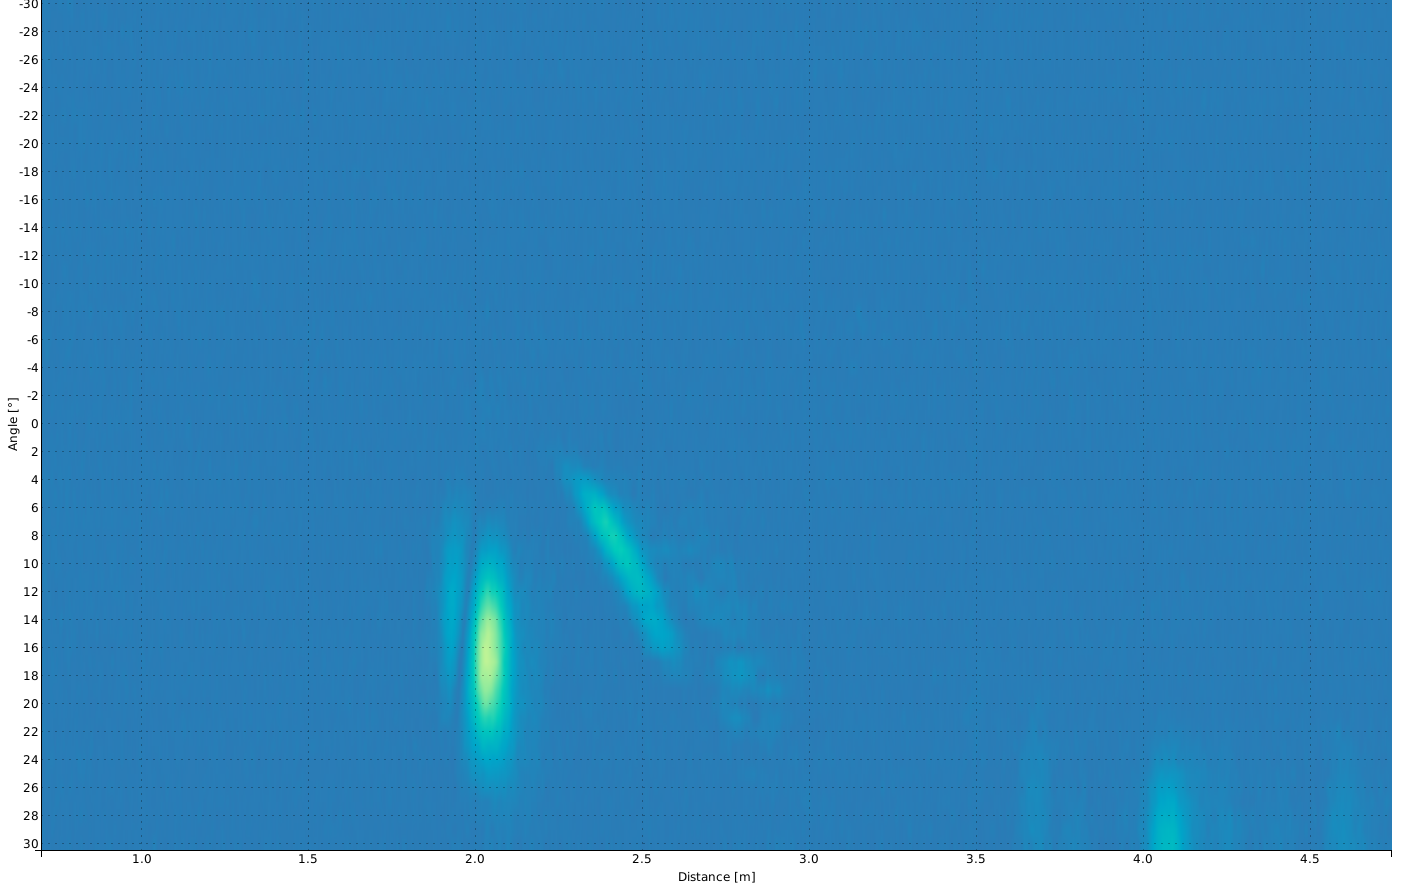
\includegraphics[width=\textwidth]{graphics/image_appendix_bild_0.png}
\caption{Styroporplatte im reflexionsarmen Halbraum, Person, die sich davon wegbewegt} % picture caption
\label{fig:image_appendix_bild_0}
%\end{figure}
%
%(Abb. \ref{fig:image1})
%%%%%%%%%%%%%%%%%%%%%%%%%%%%%%%%%%%%%%%%%%%%%%%%%%%%%%%%%%%%%%%%%%%%%%%%%%%%%%%%
\end{minipage}
\begin{minipage}{1.0\textwidth}
%%%%%%%%%%%%%%%%%%%%%%%%%%%%%%%%%%%%%%%%%%%%%%%%%%%%%%%%%%%%%%%%%%%%%%%%%%%%%%%%
% pictures
%\begin{figure}[htb]
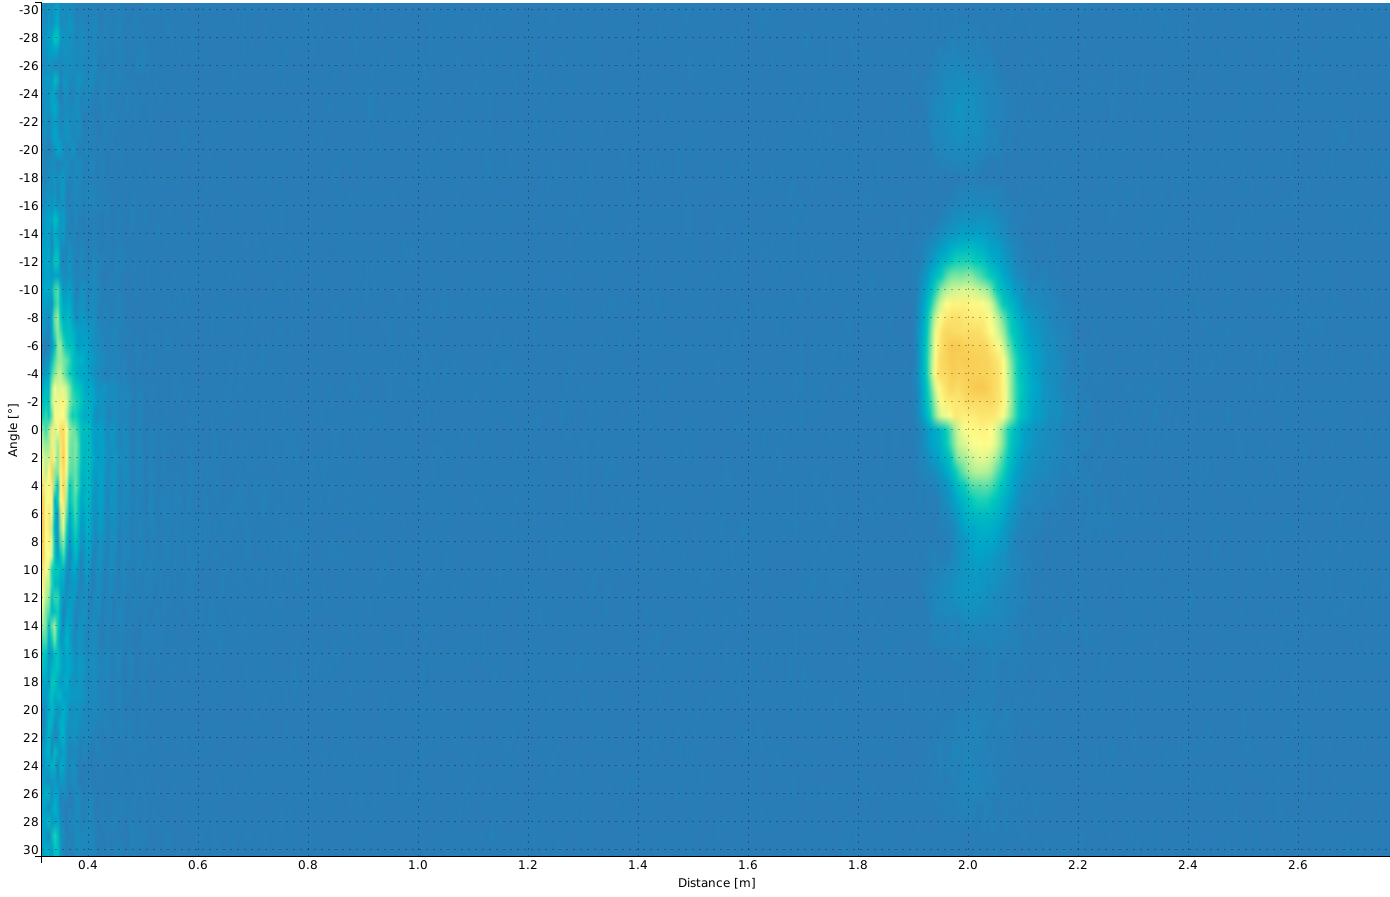
\includegraphics[width=\textwidth]{graphics/image_appendix_bild_1.png}
\caption{Styroporplatte im reflexionsarmen Halbraum, Sprung bei $0$ Grad Sendewinkel} % picture caption
\label{fig:image_appendix_bild_1}
%\end{figure}
%
%(Abb. \ref{fig:image1})
%%%%%%%%%%%%%%%%%%%%%%%%%%%%%%%%%%%%%%%%%%%%%%%%%%%%%%%%%%%%%%%%%%%%%%%%%%%%%%%%
\end{minipage}
\end{figure}


\clearpage
\begin{figure}[htb]
\begin{minipage}{1.0\textwidth}
%%%%%%%%%%%%%%%%%%%%%%%%%%%%%%%%%%%%%%%%%%%%%%%%%%%%%%%%%%%%%%%%%%%%%%%%%%%%%%%%
% pictures
%\begin{figure}[htb]
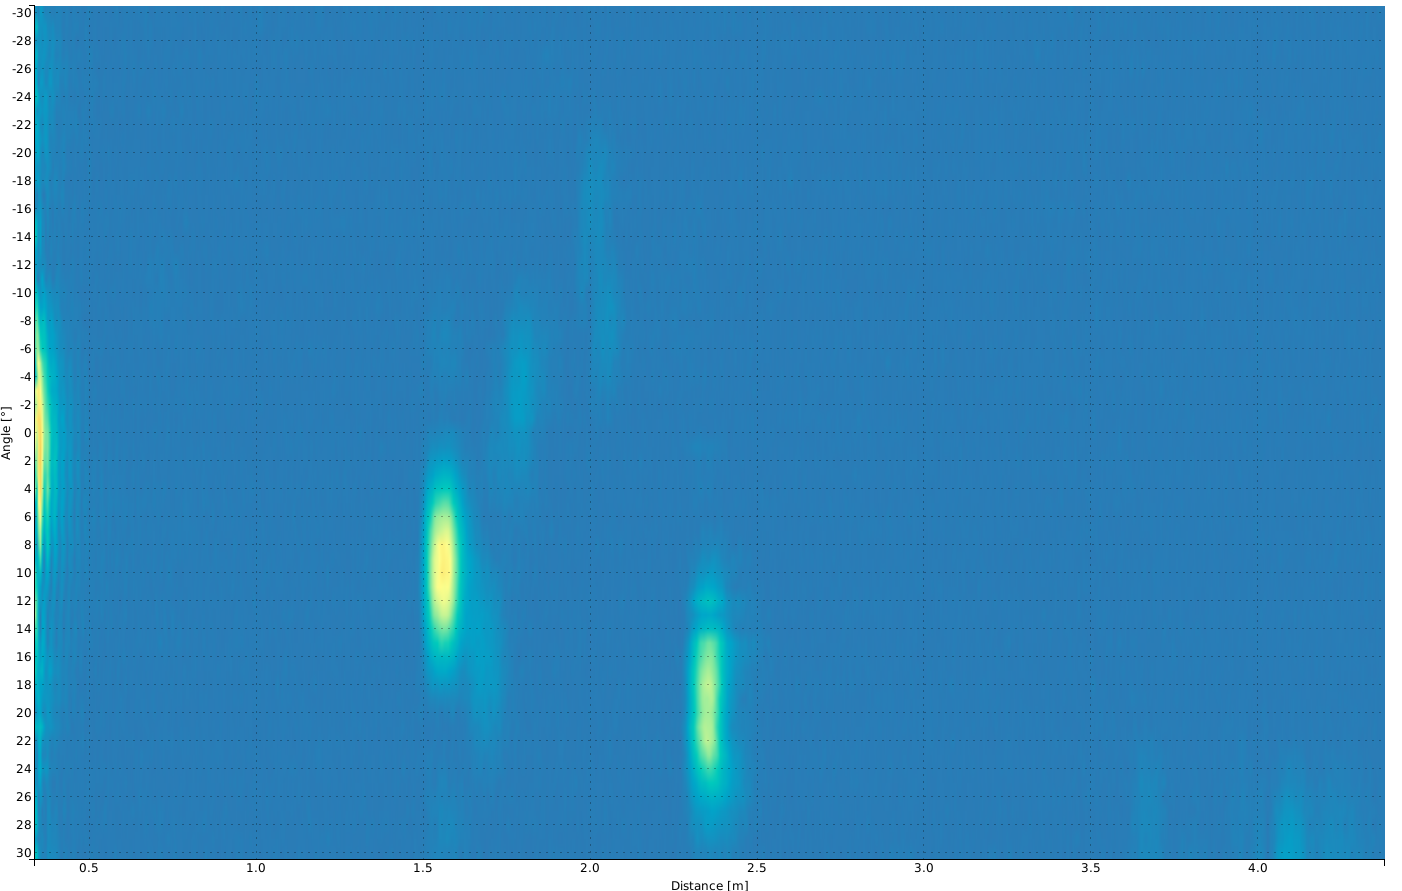
\includegraphics[width=\textwidth]{graphics/image_appendix_bild_2.png}
\caption{Aufgespanntes Tuch im reflexionsarmen Halbraum, Person steht bei $2.4 \mathrm{m}$ seitlich vom Tuch} % picture caption
\label{fig:image_appendix_bild_2}
%\end{figure}
%
%(Abb. \ref{fig:image1})
%%%%%%%%%%%%%%%%%%%%%%%%%%%%%%%%%%%%%%%%%%%%%%%%%%%%%%%%%%%%%%%%%%%%%%%%%%%%%%%%
\end{minipage}
\begin{minipage}{1.0\textwidth}
%%%%%%%%%%%%%%%%%%%%%%%%%%%%%%%%%%%%%%%%%%%%%%%%%%%%%%%%%%%%%%%%%%%%%%%%%%%%%%%%
% pictures
%\begin{figure}[htb]
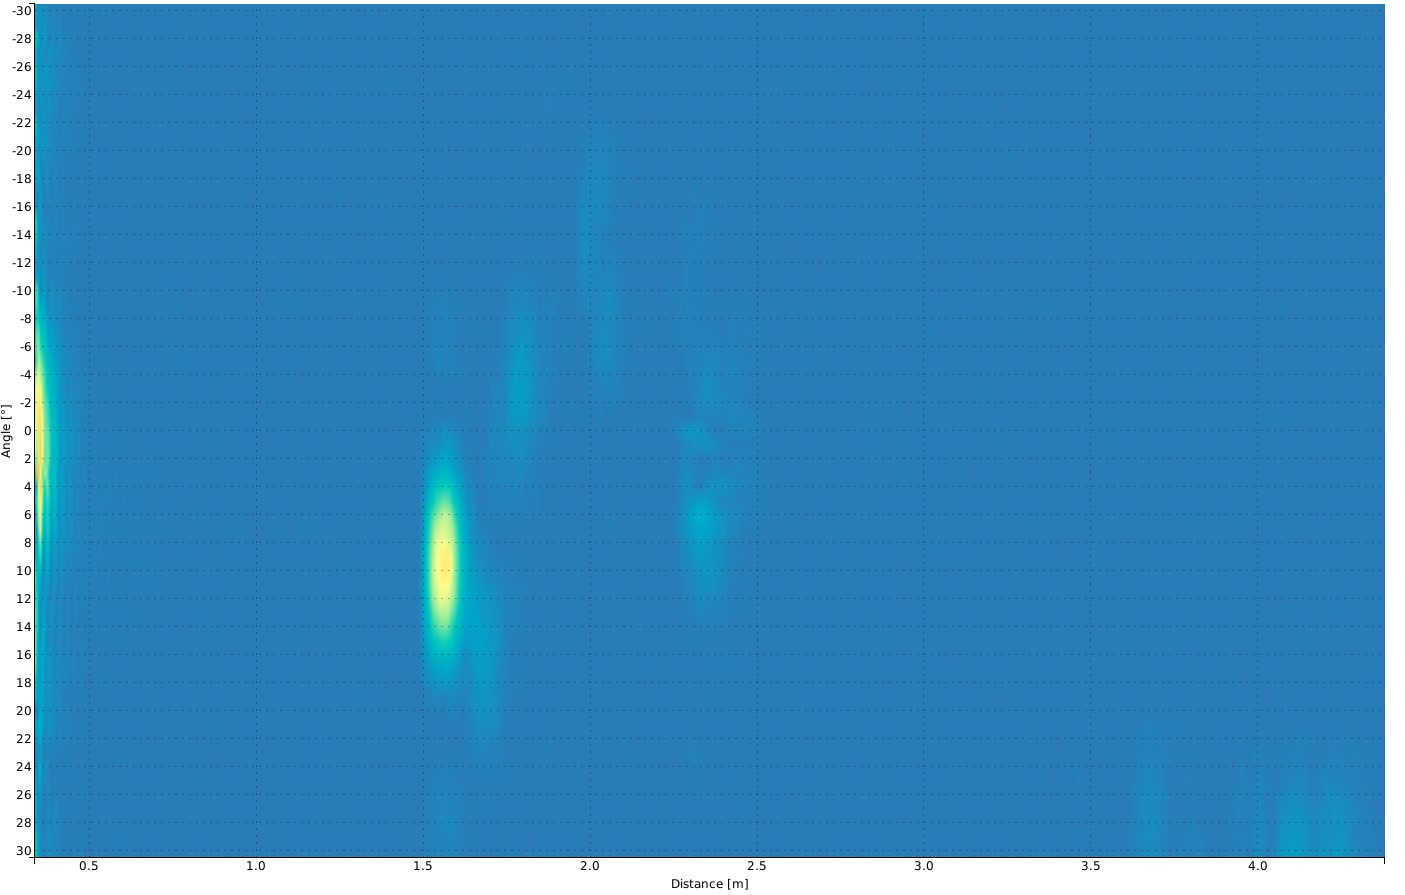
\includegraphics[width=\textwidth]{graphics/image_appendix_bild_3.png}
\caption{Aufgespanntes Tuch im reflexionsarmen Halbraum, Person steht bei $2.3 \mathrm{m}$ hinter dem Tuch} % picture caption
\label{fig:image_appendix_bild_3}
%\end{figure}
%
%(Abb. \ref{fig:image1})
%%%%%%%%%%%%%%%%%%%%%%%%%%%%%%%%%%%%%%%%%%%%%%%%%%%%%%%%%%%%%%%%%%%%%%%%%%%%%%%%
\end{minipage}
\end{figure}


\clearpage
\begin{figure}[htb]
\begin{minipage}{1.0\textwidth}
%%%%%%%%%%%%%%%%%%%%%%%%%%%%%%%%%%%%%%%%%%%%%%%%%%%%%%%%%%%%%%%%%%%%%%%%%%%%%%%%
% pictures
%\begin{figure}[htb]
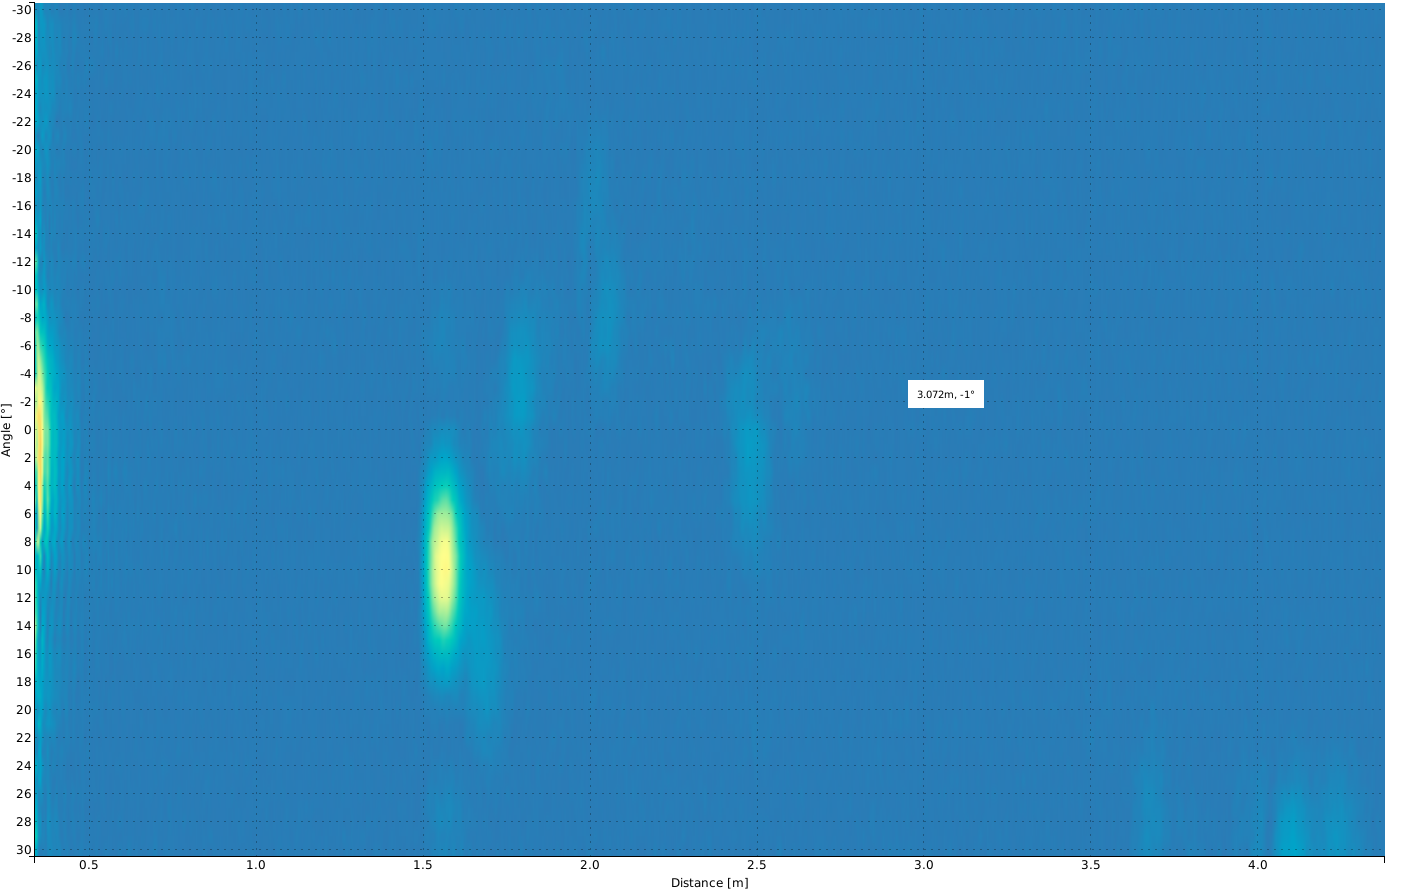
\includegraphics[width=\textwidth]{graphics/image_appendix_bild_4.png}
\caption{Aufgespanntes Tuch im reflexionsarmen Halbraum, Person steht bei $2.5 \mathrm{m}$ hinter dem Tuch} % picture caption
\label{fig:image_appendix_bild_4}
%\end{figure}
%
%(Abb. \ref{fig:image1})
%%%%%%%%%%%%%%%%%%%%%%%%%%%%%%%%%%%%%%%%%%%%%%%%%%%%%%%%%%%%%%%%%%%%%%%%%%%%%%%%
\end{minipage}
\begin{minipage}{1.0\textwidth}
%%%%%%%%%%%%%%%%%%%%%%%%%%%%%%%%%%%%%%%%%%%%%%%%%%%%%%%%%%%%%%%%%%%%%%%%%%%%%%%%
% pictures
%\begin{figure}[htb]
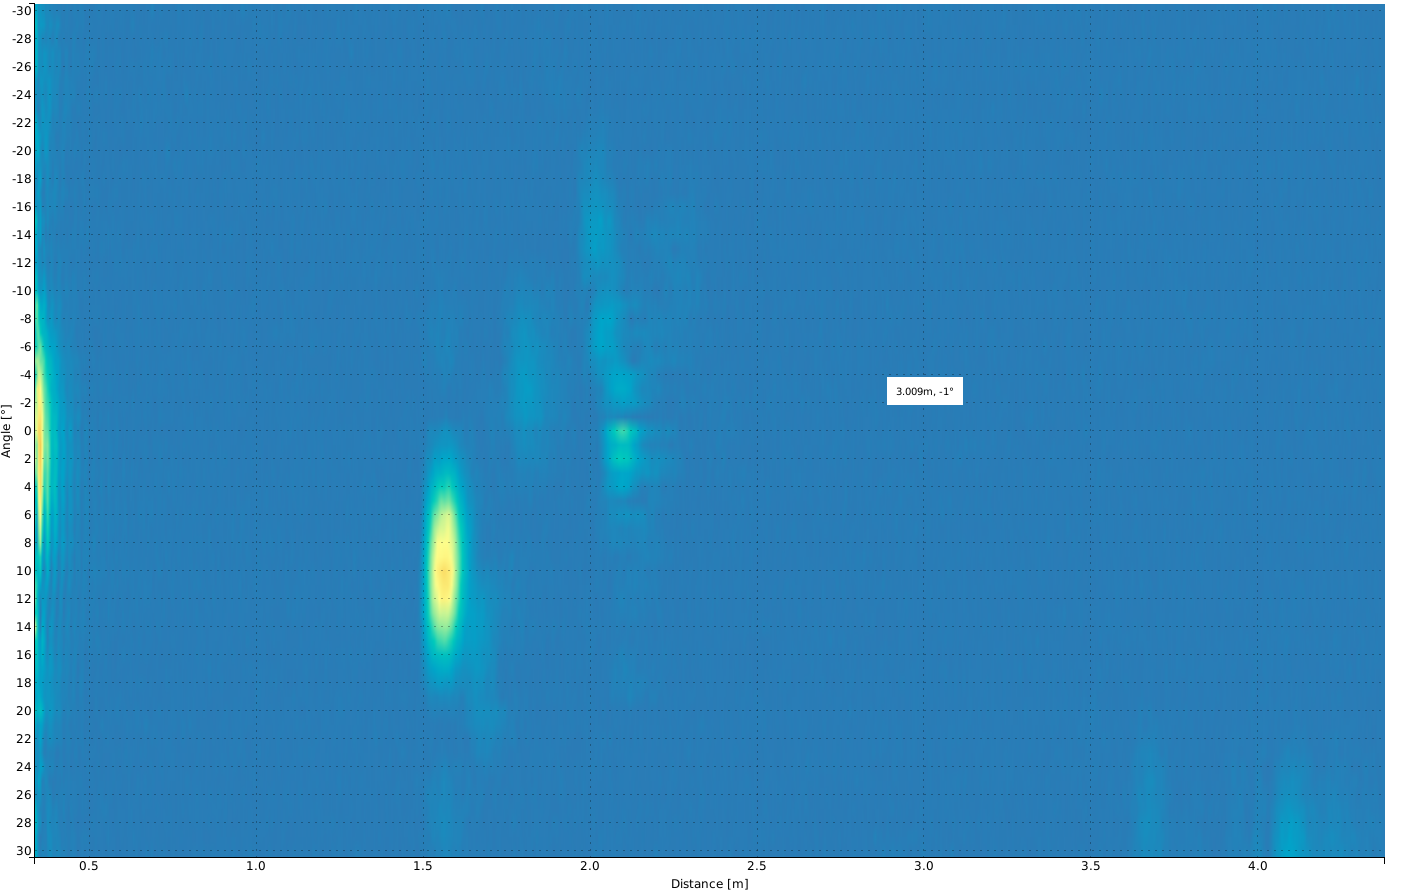
\includegraphics[width=\textwidth]{graphics/image_appendix_bild_5.png}
\caption{Aufgespanntes Tuch im reflexionsarmen Halbraum, Person steht bei $2.1 \mathrm{m}$ hinter dem Tuch} % picture caption
\label{fig:image_appendix_bild_5}
%\end{figure}
%
%(Abb. \ref{fig:image1})
%%%%%%%%%%%%%%%%%%%%%%%%%%%%%%%%%%%%%%%%%%%%%%%%%%%%%%%%%%%%%%%%%%%%%%%%%%%%%%%%
\end{minipage}
\end{figure}



\clearpage
%%%%%%%%%%%%%%%%%%%%%%%%%%%%%%%%%%%%%%%%%%%%%%%%%%%%%%%%%%%%%%%%%%%%%%%%%%%%%%%%
%%%%%%%%%%%%%%%%%%%%%%%%%%%%%%%%%%%%%%%%%%%%%%%%%%%%%%%%%%%%%%%%%%%%%%%%%%%%%%%%
%%%%%%%%%%%%%%%%%%%%%%%%%%%%%%%%%%%%%%%%%%%%%%%%%%%%%%%%%%%%%%%%%%%%%%%%%%%%%%%%
\section{Anhang Lizenzen}\label{sec:appendix_lizenzen}
Redistribution and use in source and binary forms, with or without modification, are permitted provided that the following conditions are met:
\begin{enumerate}
	\item Redistributions of source code must retain the above copyright notice, this list of conditions and the following disclaimer.
	\item Redistributions in binary form must reproduce the above copyright notice, this list of conditions and the following disclaimer in the documentation and/or other materials provided with the distribution.
	\item The name of Atmel may not be used to endorse or promote products derived from this software without specific prior written permission.
	\item This software may only be redistributed and used in connection with an Atmel microcontroller product.
\end{enumerate}

THIS SOFTWARE IS PROVIDED BY ATMEL "AS IS" AND ANY EXPRESS OR IMPLIED WARRANTIES, INCLUDING, BUT NOT LIMITED TO, THE IMPLIED WARRANTIES OF MERCHANTABILITY, FITNESS FOR A PARTICULAR PURPOSE AND NON-INFRINGEMENT ARE EXPRESSLY AND SPECIFICALLY DISCLAIMED. IN NO EVENT SHALL ATMEL BE LIABLE FOR ANY DIRECT, INDIRECT, INCIDENTAL, SPECIAL, EXEMPLARY, OR CONSEQUENTIAL DAMAGES (INCLUDING, BUT NOT LIMITED TO, PROCUREMENT OF SUBSTITUTE GOODS OR SERVICES; LOSS OF USE, DATA, OR PROFITS; OR BUSINESS INTERRUPTION) HOWEVER CAUSED AND ON ANY THEORY OF LIABILITY, WHETHER IN CONTRACT, STRICT LIABILITY, OR TORT (INCLUDING NEGLIGENCE OR OTHERWISE) ARISING IN ANY WAY OUT OF THE USE OF THIS SOFTWARE, EVEN IF ADVISED OF THE POSSIBILITY OF SUCH DAMAGE.\\


Die Sinngemässe deutsche Übersetzung dieses Lizenztextes lautet wie folgt:\\

Weitergabe und Verwendung in Sourcecode oder kompilierter Form, mit oder ohne Veränderungen, sind erlaubt solange folgende Bedingungen eingehalten werden:
\begin{enumerate}
	\item Weitergegebener Sourcecode muss das obenstehende Copyright, diese Auflistung von Vereinbarungen, sowie den nachfolgenden Hinweis enthalten.
	\item Weitergegebene Software in kompilierter Form muss das obenstehende Copyright, diese Auflistung von Vereinbarungen, sowie den nachfolgenden Hinweis in der Dokumentation und/oder anderen mit der Software verteilten Bestandteilen des Produktes enthalten.
	\item Ohne explizite schriftliche Erlaubnis darf der Name von Atmel nicht verwendet werden, um das von dieser Software abgeleitete Produkt zu bewerben.
	\item Diese Software darf nur weitergegeben und benutzt werden in Verbindung mit einem Atmel Mikrocontroller Produkt.
\end{enumerate}

DIESE SOFTWARE WIRD VON ATMEL ZUR VERFÜGUNG GESTELLT OHNE JEGLICHE DIREKTE ODER IMPLIZIERTE GARANTIE AUF FUNKTIONSFÄHIGKEIT FÜR EINEN BESTIMMTEN ZWECK, DIE FUNKTIONSFÄHIGKEIT ALLGEMEIN, SOWIE JEGLICHER RECHTSVERLETZUNG, JEDOCH NICHT DARAUF BESCHRÄNKT. IN KEINEM FALL IST ATMEL HAFTBAR FÜR JEGLICHEN DIREKTEN, INDIREKTEN, UNBEABSICHTIGTEN, SPEZIELLEN, EXEMPLARISCHEN ODER FOLGESCHADEN (INKLUSIVE, ABER NICHT BESCHRÄNKT AUF DIE BESCHAFFUNG VON ERSATZGÜTERN ODER DIENSTLEISTUNGEN; NUTZUNGSAUSFALL, DATENVERLUST ODER PROFITVERLUST; ODER BETRIEBSAUSFALL) WIE AUCH IMMER VERURSACHT UND UNABHÄNGIG VON DER RECHTSGRUNDLAGE DER HAFTUNG, OB VERTRAGLICH, IN VERSCHULDUNGSUNABHÄNGIGER HAFTUNG, ODER AUS UNERLAUBTER HANDLUNG (EINSCHLIESSLICH FAHRLÄSSIGKEIT ODER ANDERE), WELCHE AUF JEGLICHE ART DURCH DEN GEBRAUCH DER SOFTWARE AUFTRITT, SOGAR WENN AUF DIE MÖGLICHKEIT EINES SOLCHEN SCHADENS HINGEWIESEN WURDE.



\clearpage
%%%%%%%%%%%%%%%%%%%%%%%%%%%%%%%%%%%%%%%%%%%%%%%%%%%%%%%%%%%%%%%%%%%%%%%%%%%%%%%%
%%%%%%%%%%%%%%%%%%%%%%%%%%%%%%%%%%%%%%%%%%%%%%%%%%%%%%%%%%%%%%%%%%%%%%%%%%%%%%%%
%%%%%%%%%%%%%%%%%%%%%%%%%%%%%%%%%%%%%%%%%%%%%%%%%%%%%%%%%%%%%%%%%%%%%%%%%%%%%%%%
\section{Anhang Aufgabenstellung}\label{sec:appendix_aufgabenstellung}
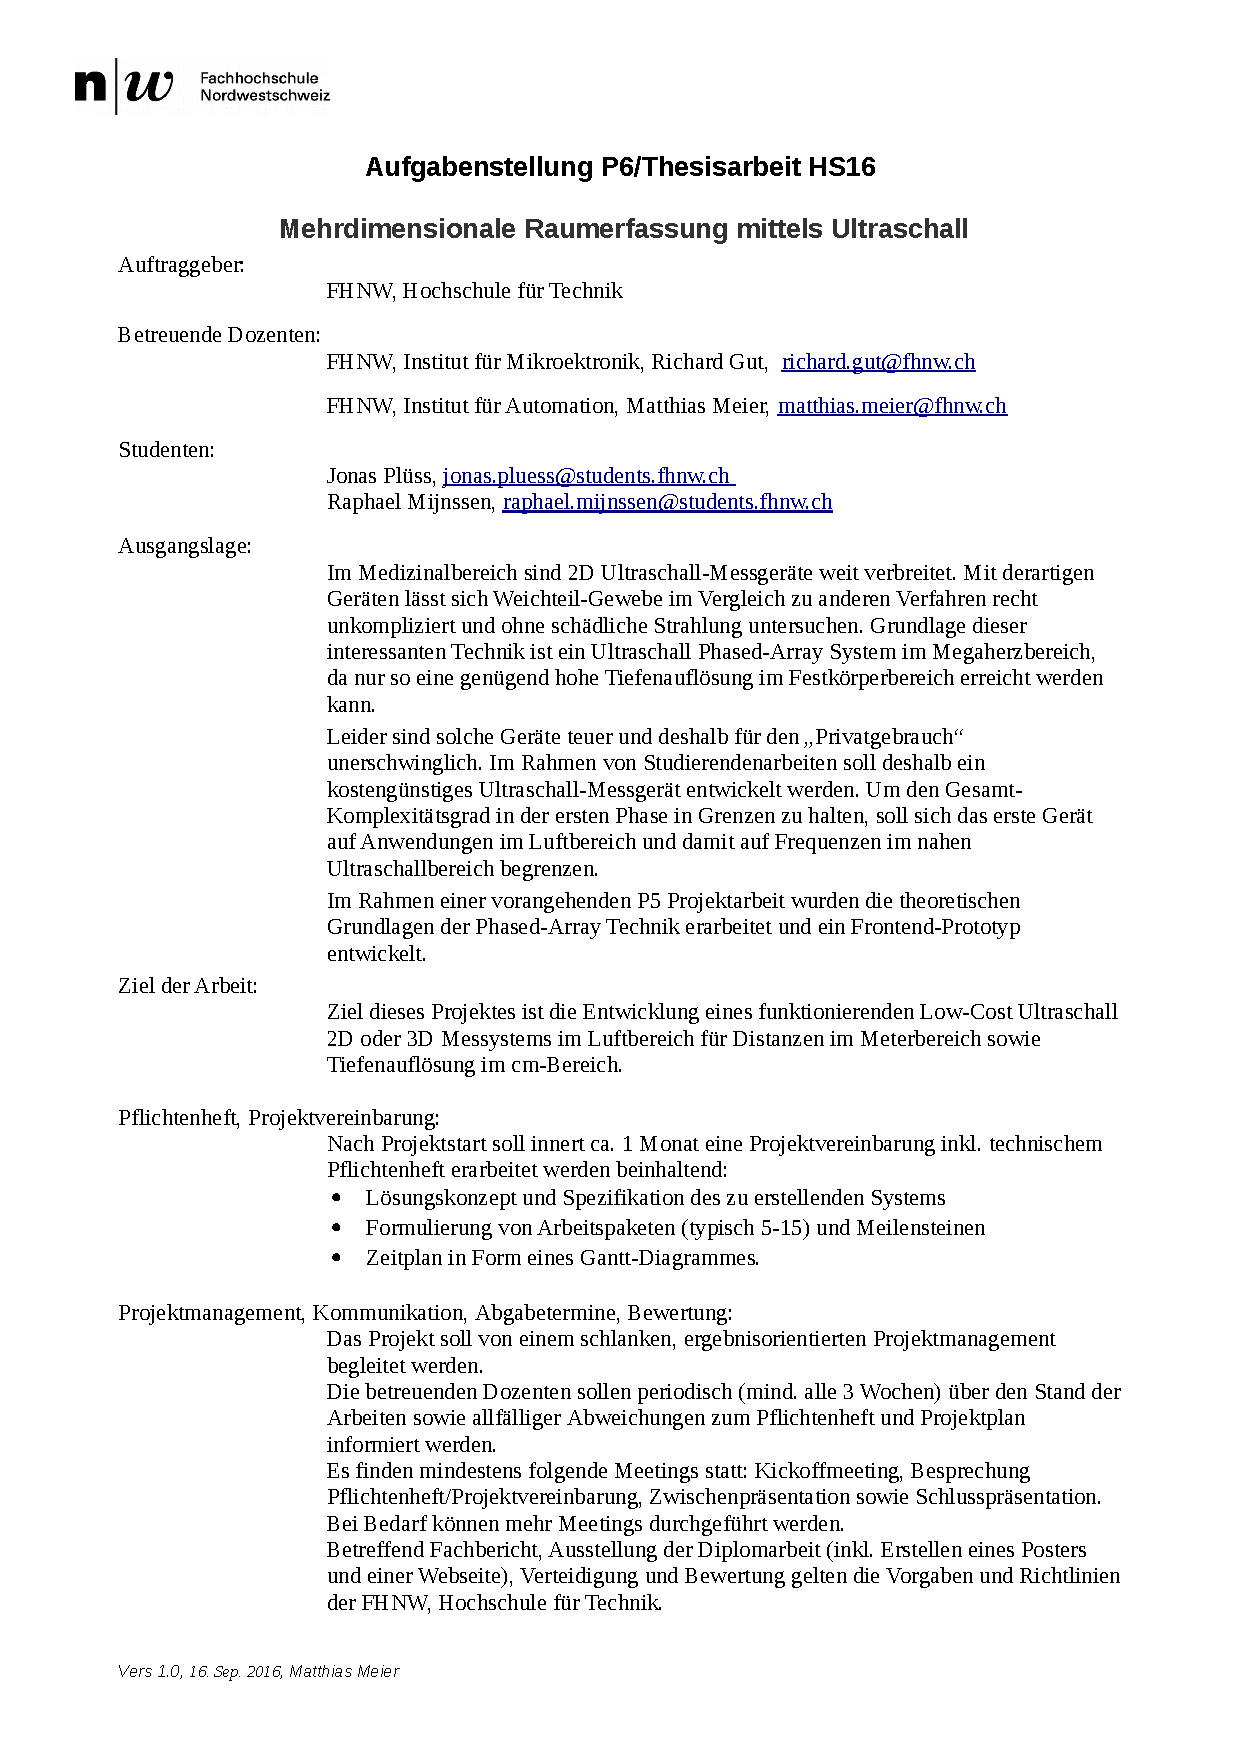
\includepdf[pages={-}]{appendix/aufgabenstellung.pdf}



\clearpage
%%%%%%%%%%%%%%%%%%%%%%%%%%%%%%%%%%%%%%%%%%%%%%%%%%%%%%%%%%%%%%%%%%%%%%%%%%%%%%%%
%%%%%%%%%%%%%%%%%%%%%%%%%%%%%%%%%%%%%%%%%%%%%%%%%%%%%%%%%%%%%%%%%%%%%%%%%%%%%%%%
%%%%%%%%%%%%%%%%%%%%%%%%%%%%%%%%%%%%%%%%%%%%%%%%%%%%%%%%%%%%%%%%%%%%%%%%%%%%%%%%
\section{Anhang Pflichtenheft}\label{sec:appendix_pflichtenheft}
\includepdf[pages={-}]{appendix/pflichtenheft.pdf}
